\section{Data}
\label{sec:data}

\subsection{Dataset, Preselection and Mass}
\label{sec:data_presel}
\emph{In short: $8{,}556{,}118$ candidates are reduced to $23{,}895$ by a kaon-identification and muon-veto requirement common to the analyses; the fit window $[5100,5600]\,\MeV$ contains $19{,}731$ candidates ($10{,}292$ $B^+$, $9439$ $B^-$).}
The dataset is the CERN Open Data record 4900~\cite{opendata_record}: $B^{\pm}\to h^{\pm}h^{+}h^{-}$ candidates collected by LHCb in 2011 at $\sqrt{s}=7$\,TeV, already through trigger and offline selection, split by magnet polarity ($8{,}556{,}118$ candidates), and a phase-space simulation of $B^{\pm}\to K^{\pm}K^{+}K^{-}$ ($50{,}000$ decays, no asymmetry) used only to test the local-asymmetry procedure (Sec.~\ref{sec:dalitz}). The same preselection is used in all analyses,
\[
\texttt{H*\_ProbPi} < 0.5 \ \wedge\ \texttt{H*\_ProbK} > 0.5 \ \wedge\ \lnot\texttt{H*\_isMuon},
\]
for each of the three tracks, and retains $23{,}895$ candidates ($0.28\%$); the cut flow is in Table~\ref{tab:cutflow} of Appendix~\ref{app:ext_data}. $H1$ is always the kaon of charge opposite to the $B$, so the Dalitz variables are $m^2(H1,H2)$ and $m^2(H1,H3)$.

\label{sec:data_mass}
The three tracks are assigned the charged-kaon mass and their four-momenta are summed to reconstruct $m(KKK)$. The nominal fit window, common to the two analyses, is $[5100,5600]\,\MeV$ and contains $19{,}731$ candidates ($11{,}636$ magnet down, $8095$ magnet up). Below $\sim$5150\,\MeV\ the background rises, which a single exponential cannot describe; the window includes the start of this rise, described by a second exponential in the background model (Secs.~\ref{sec:frequentist}--\ref{sec:bayesian}).

\subsection{Data Exploration}
\label{sec:data_exploration}
\emph{In short: the spectrum peaks at $5284\,\MeV$ with a similar shape for the two charges and the two magnet polarities, and the counting asymmetry of all candidates is $-0.043\pm0.007$.}
\begin{figure*}[t]
\centering
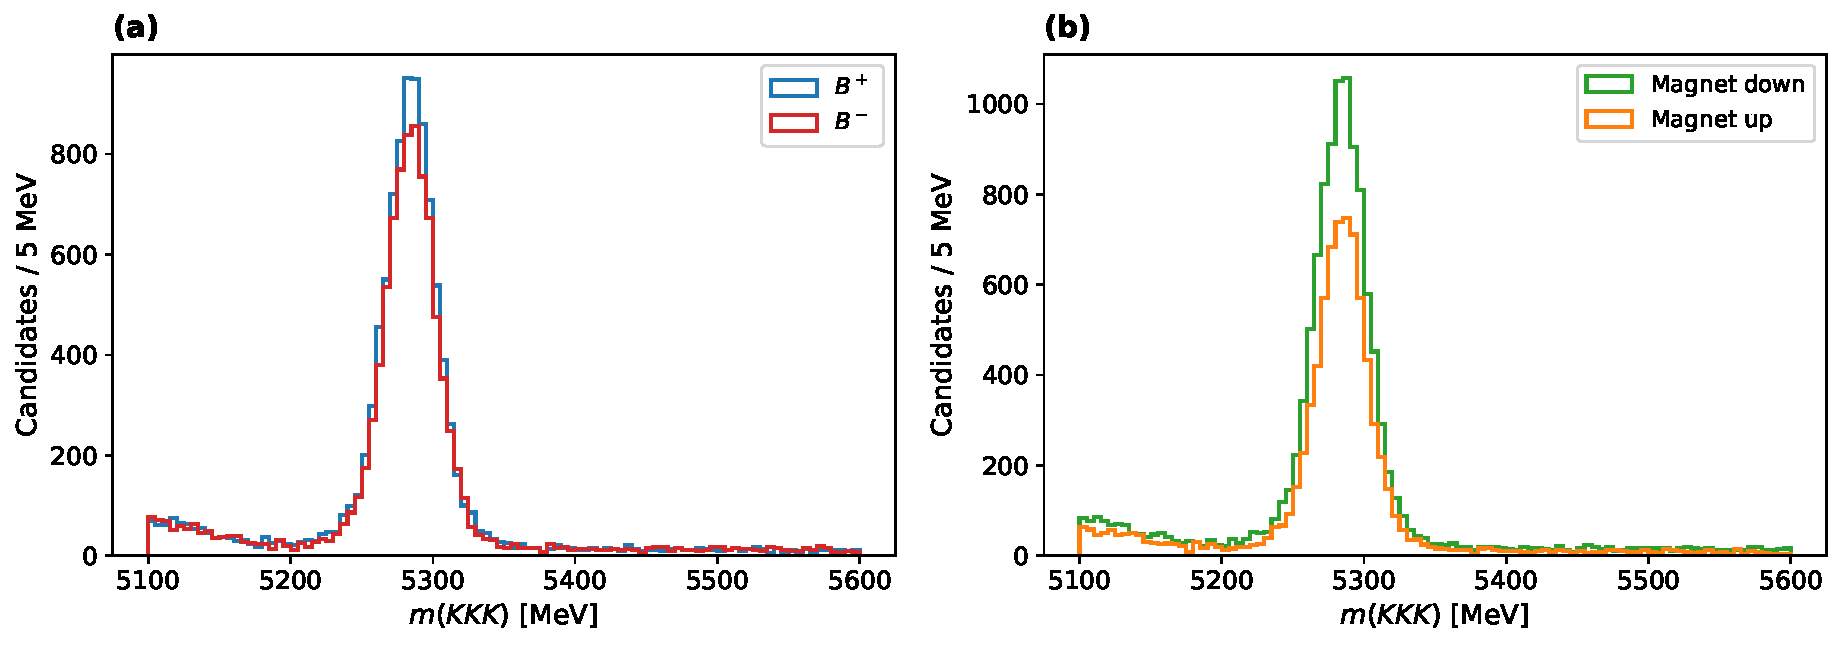
\includegraphics[width=0.95\textwidth]{figures/mass_spectrum.pdf}
\caption{Reconstructed $B\to KKK$ invariant mass in the nominal fit window $[5100,5600]\,\MeV$, split by (a) $B$ charge and (b) magnet polarity. Both splits show a consistent peak at $m\approx5284\,\MeV$ over a falling combinatorial background, which rises below $\sim$5150\,\MeV.}
\label{fig:mass_spectrum}
\end{figure*}

Figure~\ref{fig:mass_spectrum} shows the spectrum in the fit window. The peak at $m\approx5284\,\MeV$ over a falling combinatorial background has the same shape for the two charges and the two polarities, which allows a mass and a resolution common to $B^+$ and $B^-$ in the model (Sec.~\ref{sec:model}). The counting asymmetry of all candidates, signal and background together, is $A_{\mathrm{count}}=(N^--N^+)/(N^-+N^+)=-0.043\pm0.007$ (binomial uncertainty); the fits of Secs.~\ref{sec:frequentist} and \ref{sec:bayesian} refine it by separating signal and background.
